\centering


\usetikzlibrary{shapes, arrows}

\tikzstyle{block} = [draw, rectangle, minimum width = 0.75cm, minimum height = 0.75cm]
\tikzstyle{sum} = [draw, circle, minimum size=.5cm, node distance=1.75cm]
\tikzstyle{input} = [coordinate]
\tikzstyle{output} = [coordinate]
\tikzstyle{support} = [coordinate]

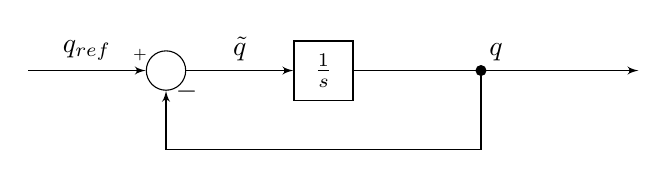
\begin{tikzpicture}[node distance=2cm,auto,>=latex']
\node [input, name=input] {};
\node [sum, right of=input] (sum) {};
\node [block, right of=sum] (int1) {$\frac{1}{s}$};
\node [support, right of=int1](s1){};
\node [output, right of=s1] (output) {}; 
\node [input, below of=int1] (feedback) {}; 

\draw [->] (input) -- node[name = qin] {{$q_{ref}$}} node[pos=0.95] {{\tiny $+$}} (sum);
\draw [->] (sum) -- node[name = qer] {{$\tilde{q}$}} (int1);
\draw [->] (int1) -- node[name = q] {{$q$}} (output);
\draw [->](s1) -- +(0,-1) -| node[pos=0.99, right] {{$-$}} (sum);


\fill (s1) circle [radius=2pt];
\end{tikzpicture}